\documentclass[border=10pt]{standalone}
% Shared preamble for the VibeStack report diagrams.
% Build one diagram: pdflatex fig_x.tex && pdftoppm -r 220 -png -singlefile fig_x.pdf ../images/fig_x
\usepackage[T1]{fontenc}
\usepackage{lmodern}
\renewcommand{\familydefault}{\sfdefault}
\usepackage{tikz}
\usetikzlibrary{arrows.meta,positioning,shapes.geometric,shapes.misc,fit,backgrounds,calc}
\definecolor{vsred}{RGB}{204,0,0}
\definecolor{lay1}{RGB}{232,240,254}
\definecolor{lay2}{RGB}{230,246,236}
\definecolor{lay3}{RGB}{255,243,224}
\definecolor{lay4}{RGB}{243,232,253}
\tikzset{
  box/.style={draw, rounded corners=3pt, align=center, minimum height=0.95cm, inner sep=5pt, fill=white, font=\small},
  sbox/.style={box, minimum width=2.6cm},
  arrow/.style={-{Stealth[length=2.4mm]}, thick},
  darrow/.style={arrow, dashed},
  lbl/.style={font=\scriptsize, fill=white, inner sep=1.5pt},
  decision/.style={draw, diamond, aspect=2.1, align=center, inner sep=1pt, font=\small, fill=white},
  term/.style={draw, rounded rectangle, minimum width=2.4cm, minimum height=0.9cm, font=\small\bfseries, fill=white},
}

\begin{document}
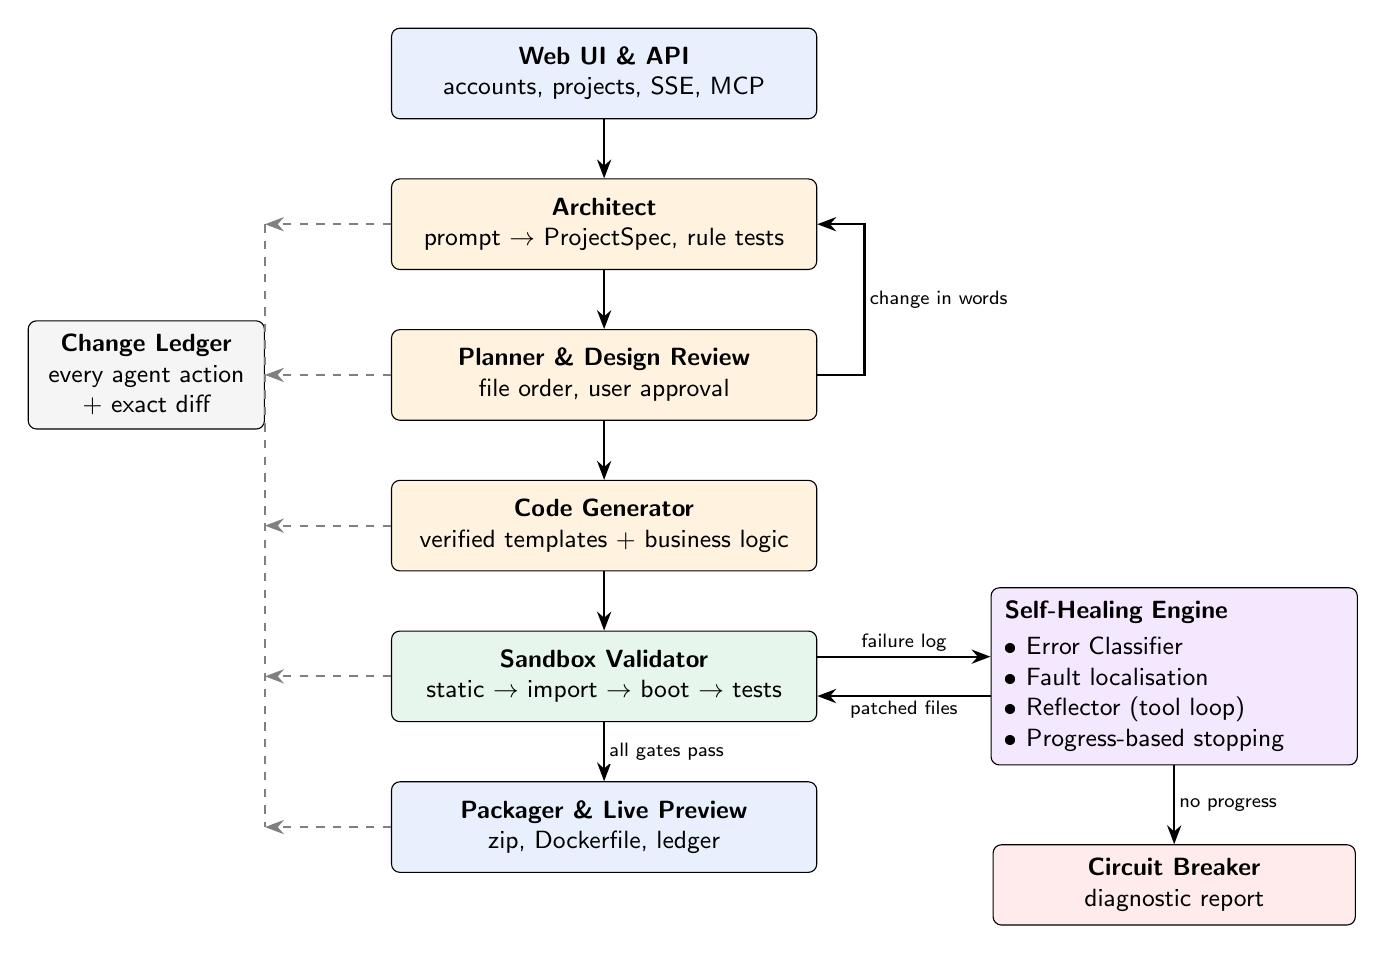
\begin{tikzpicture}[node distance=0.75cm]
\tikzset{mbox/.style={box, minimum width=5.4cm, minimum height=1.15cm}}
\node[mbox, fill=lay1] (ui) {\textbf{Web UI \& API}\\accounts, projects, SSE, MCP};
\node[mbox, fill=lay3, below=of ui] (arch) {\textbf{Architect}\\prompt $\rightarrow$ ProjectSpec, rule tests};
\node[mbox, fill=lay3, below=of arch] (plan) {\textbf{Planner \& Design Review}\\file order, user approval};
\node[mbox, fill=lay3, below=of plan] (gen) {\textbf{Code Generator}\\verified templates + business logic};
\node[mbox, fill=lay2, below=of gen] (val) {\textbf{Sandbox Validator}\\static $\rightarrow$ import $\rightarrow$ boot $\rightarrow$ tests};
\node[mbox, fill=lay1, below=of val] (pack) {\textbf{Packager \& Live Preview}\\zip, Dockerfile, ledger};
\node[box, fill=lay4, right=2.2cm of val, minimum width=4.6cm, align=left, text width=4.3cm] (heal) {\textbf{Self-Healing Engine}\\[2pt]
\textbullet\ Error Classifier\\ \textbullet\ Fault localisation\\ \textbullet\ Reflector (tool loop)\\ \textbullet\ Progress-based stopping};
\node[box, fill=red!8, below=1.0cm of heal, minimum width=4.6cm] (cb) {\textbf{Circuit Breaker}\\diagnostic report};
\node[box, fill=gray!8, left=1.6cm of plan, minimum width=3cm] (ledger) {\textbf{Change Ledger}\\every agent action\\+ exact diff};
\foreach \a/\b in {ui/arch, arch/plan, plan/gen, gen/val} \draw[arrow] (\a) -- (\b);
\draw[arrow] (val) -- node[lbl, right]{all gates pass} (pack);
\draw[arrow] (val.east) ++(0,0.25) -- node[lbl, above]{failure log} ($(heal.west)+(0,0.25)$);
\draw[arrow] ($(heal.west)+(0,-0.25)$) -- node[lbl, below]{patched files} ($(val.east)+(0,-0.25)$);
\draw[arrow] (heal) -- node[lbl, right]{no progress} (cb);
\draw[arrow] (plan.east) -- ++(0.6,0) |- node[lbl, pos=0.25, right]{change in words} (arch.east);
\foreach \n in {arch, plan, gen, val, pack} \draw[darrow, gray] (\n.west) -- (ledger.east |- \n.west);
\draw[gray, thick, dashed] (ledger.east |- arch.west) -- (ledger.east |- pack.west);
\end{tikzpicture}
\end{document}
